\section{Použití trezoru}
Mechanické verze trezoru M1 a M2 měli na akcích a v kroužcích dětmi možnost trezor jen stavět. První akce založená na trezoru, která neobsahovala jen stavbu, využívala už variantu M3.
Protože na akci byli menší děti místo klasické číselné stupnice byl trezor vybaven obrázkovým kódem jak je vidět na obrázku \ref{fig:M3-trpaslici}.

\begin{figure}[htbp]
    \centering
    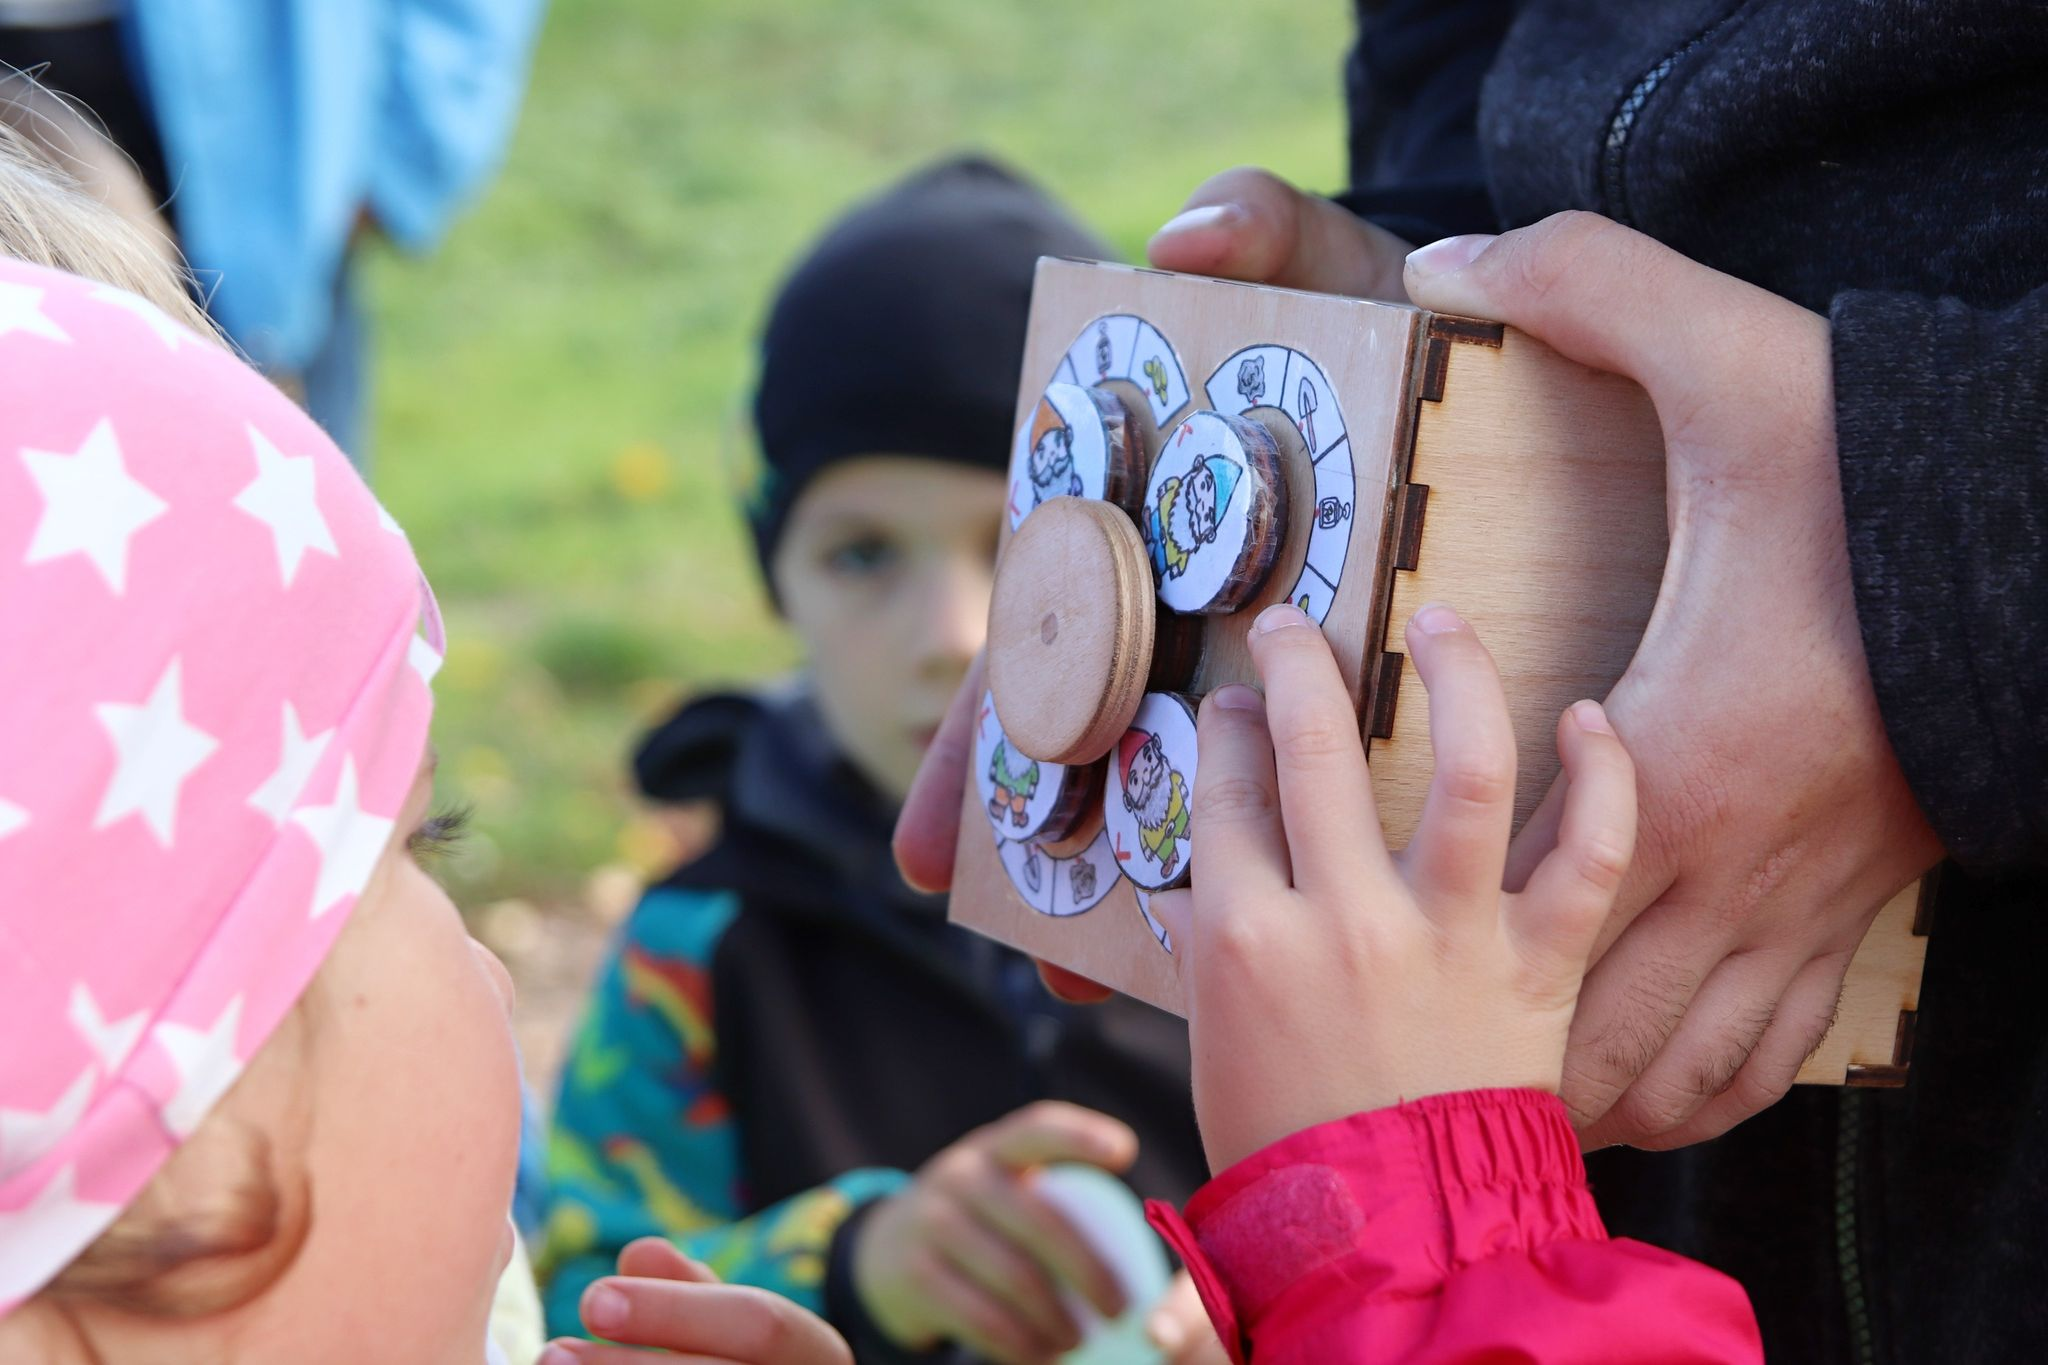
\includegraphics[width=\textwidth]{kapitoly/obrazky/M3/trpaslici.png}
    \caption{Render varianty M3}
    \label{fig:M3-trpaslici}
\end{figure}
